\documentclass[letterpaper,twoside]{article}
\usepackage[T1]{fontenc}
\usepackage{textcomp}
\usepackage{mathptmx}
\usepackage[scaled=0.9]{helvet}
\usepackage{url}
\usepackage{graphicx}
\setcounter{secnumdepth}{-2}
\title{Web Librarian Plugin User Manual}
\author{Robert Heller}
\date{\today}
\begin{document}

\maketitle

\tableofcontents

\section{Introduction}

This WordPress plugin started as a portable, cross-platform system that
the Wendell Free Library could use as a transistion system from its current
paper card based circulation system to the system that will eventually
be rolled out by the regional library system.  It has `morphed' to a
web-based successor to Deepwoods Software's Home Librarian 3 system.

This plugin implements a simple and basic, web-based, library catalog
and circulation system.  There are short codes that can be added to
pages of a WordPress site to search and display items in the library
collection.  And there are back-end (admin) pages that implement
managment of the collection, management of patrons (users) of the
library, as well as implementing the functionallity of a  circulation
desk. 

\section{Installation and basic setup}

The plugin can be installed by uploading the Zip
file\footnote{Eventually I'll upload this plugin to the WordPress
plugin repository, at which point it will be available for automatic
installation and updating.}.

There are some options that can be set, but these options are not needed
for basic operation.  

\subsection{Option Settings}

There are three options, all of which relate to Amazon's Web Services.
If you want to be able to lookup product information about items you
add to your collection, you should sign up with Amazon and get a set of
Amazon Web Services public and private keys.  You also need an Amazon
Associate Tag as well. Once you have these keys, you would set them
with the Web Librarian's option settings:
\begin{enumerate}
\item \textbf{AWS Public Key} This is your Amazon Web Services public key.
\item \textbf{AWS Private Key} This is your Amazon Web Services private key.
\item \textbf{AWS Region} This is your Amazon Web Services region.
\item \textbf{Amazon Associate Tag} This is your Amazon Associate Tag.
\end{enumerate}
All \textbf{four} options are required to use the Amazon item lookup features.

\subsection{User Role Setup}

The Web Librarian adds three priviledges:

\begin{enumerate}
\item \textbf{manage\_patrons} This allows adding, removing, and editing
patrons.
\item \textbf{manage\_collection} This allows adding, removing, and
editing items in the collection.
\item \textbf{manage\_circulation} This allows basic circulation tasks,
such as checking out items, checking in items, and placing holds on items.
\end{enumerate}

And three roles:
\begin{enumerate}
\item \textbf{Librarian} The librarian role gets all of the above
privledges, plus \textbf{edit\_users}\footnote{Needed to associate
patron ids with users.}. Typically the senior librarian or library
directory gets this role.
\item \textbf{Senior Aid} The senior aid gets the
\textbf{manage\_collection} and \textbf{manage\_circulation} privledges,
which allows a senior aid to both add, edit, and remove items from the
collection as well as perform circulation tasks.
\item \textbf{Volunteer} The volunteer only gets the
\textbf{manage\_circulation} privledge, which allows the volunteer to
run the circulation desk.
\end{enumerate}

For a typical small library, only the senior librarian or library
director has the authority to add, edit, or remove library
patrons, that is issue, alter, or revoke library lending access. A
senior aid would be an assistant librarian who is authorized to do both
circulation desk duty and to enter or remove items from the collection,
which is more of a back office task.  Volunteers would be people who
would man the circulation desk and check items out and possibly check returned
items back in.  For a very small library, there might be only one person
and that person would be the senior librarian.  Note this is a separate
user from the site administrator.

\subsection{Short codes for front side access to the collection}

To make the collection searchable and visible on the front side of your
blog, you will need to create pages with one or more of the supplied
short codes.  Three short codes are defined:
\begin{enumerate}
\item \textbf{weblib\_searchform} This short code generates a collection
search form  It takes these parameters:
  \begin{description}
  \item[name] The name to use for the form. The default is `searchform'.
  \item[actionurl] The action URL for the form. The default is `'
(implies that the current page will generate the search results).
  \item[method] The form method. The default is `GET'.
  \end{description}
The search form allows searching by Title, Author, Subject, Keyword, or
ISBN. The results can be ordered by System Sorted (barcode order), Title
or by Author, either in Ascending or Descending order.

The form passes to the action page these parameters:
\begin{description}
\item[searchby] The field to search on, one of title, author, subject,
keyword, or isbn,
\item[searchbox] The search text.
\item[weblib\_orderby] The field to sort the results with, one of
barcode, title, or author.
\item[weblib\_order] The sort order to use, one of ASC or DESC.
\end{description}
\item \textbf{weblib\_itemlist} This short code generates a list of
results. It will process the parameters generated by the
\textbf{weblib\_searchform} short code.  It takes these parameters:
  \begin{description}
  \item[name] The name to use for the item list div. The default is `itemlist'.
  \item[per\_page] The number of items to display on each page. The
default is 10.
  \item[moreinfourl] The URL of the page where more info on a selected
item is displayed. The default is `'. 
  \item[inlinemoreinfo] A flag, if true, that will cause this short code
to display more information on a selected item. The default is false.
  \item[holdbutton] A flag, if true and if the logged in user has a
patron id, will include a button to request a hold on items. The
default is false.
  \end{description}
This short code calls the \textbf{weblib\_itemdetail} short code to
generate brief displays of matched items or (if \textbf{inlinemoreinfo}
is true) to generate a long display of a selected item (or if only one
item matches). 
\item \textbf{weblib\_itemdetail} This short code displays one item in
greater or lesser detail. It would generally be on a page by itself
(typically the target of the \textbf{moreinfourl} passed to
\textbf{weblib\_itemlist}). It takes these parameters:
  \begin{description}
  \item[name] The name of the enclosing div.  The default is
`itemdetail[\%i]', where \%i is replaced by the item's barcode.
  \item[barcode] The barcode of the item to display. The default is `'.
  \item[getbarcode] A flag, if true, that causes this short code to get
the barcode from the CGI parameters. Typically used with the
\textbf{moreinfourl} parameter of the \textbf{weblib\_itemlist} short
code. The default is true.
  \item[holdbutton] A flag, if true and if the logged in user has a
patron id, will include a button to request a hold on items. The
default is false.
  \item[detaillevel] The level of detail to display. Setting this to
`brief' (the default) causes a brief level of detail, suitable in a
listing of several items (this is what the \textbf{weblib\_itemlist}
short code uses when displaying multiple results).  Setting this to
`long' cause a more detailed level of display (this is what the
\textbf{weblib\_itemlist} short code uses when displaying a single item
in detail).
  \item[moreinfourl] The URL of the page where more info on a selected
item is displayed. The default is `'. 
  \end{description}
This short code is invoked by the \textbf{weblib\_itemlist} short code
and this short code is not actually needed on its own, unless you wish
to highlight a selected item or items on a page of their own.
\end{enumerate}

\subsubsection{A basic example}

\begin{figure}[htbp]
\begin{centering}
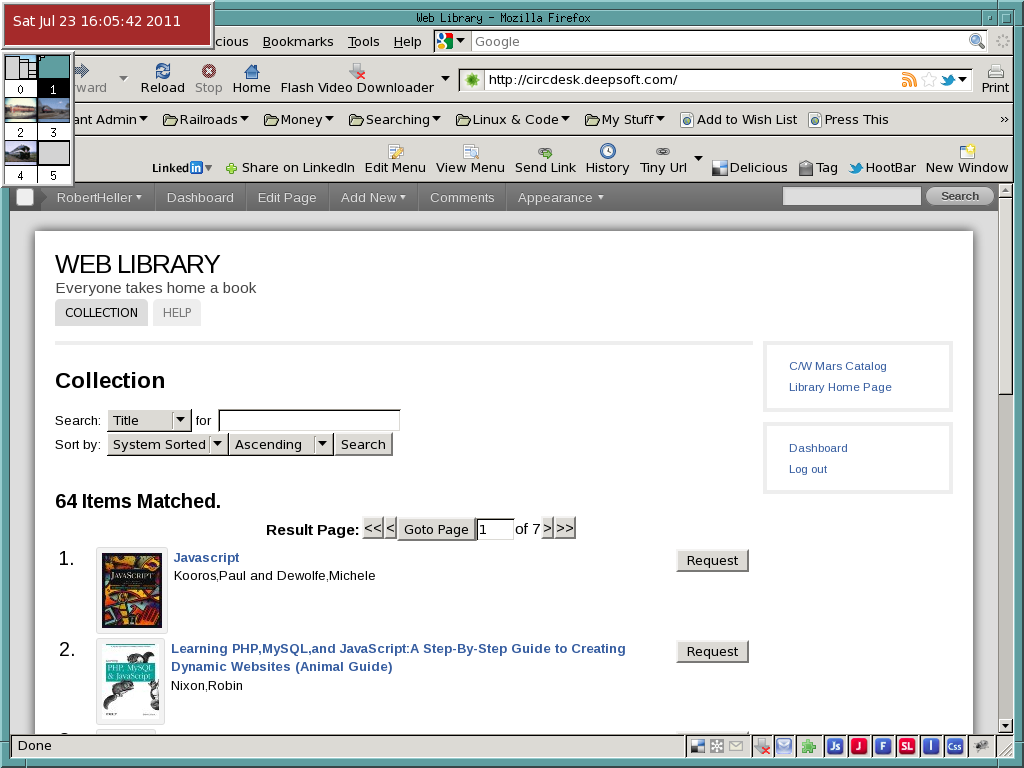
\includegraphics[width=4in]{frontside.png}
\caption{Front side view of the basic short code content -- list of brief results}
\label{fig:frontside}
\end{centering}
\end{figure}
\begin{figure}[htbp]
\begin{centering}
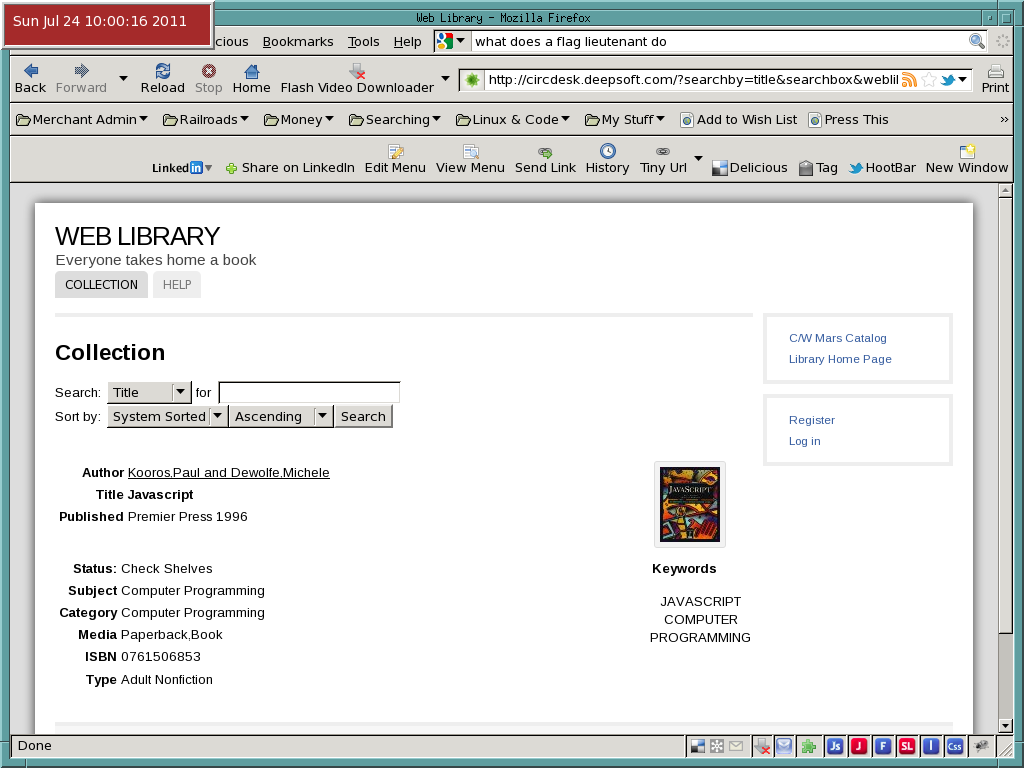
\includegraphics[width=4in]{frontone.png}
\caption{Front side view of the basic short code content -- one item in long form}
\label{fig:frontone}
\end{centering}
\end{figure}
A page containing just the following content is enough to provide a
search and display of items in your library collection. The results of
this page are shown in Figures~\ref{fig:frontside} and \ref{fig:frontone}.

\begin{verbatim}
[weblib_searchform]
[weblib_itemlist holdbutton=1 inlinemoreinfo=1]
\end{verbatim}



\section{Profile / User Management}

This plugin adds several pages to the user management / profile
dashboard pages, upto 3 for non-priviledged users and upto 4 for users
with `edit\_user' priviledge.  These pages are:
\begin{enumerate}
\item \textbf{Edit Patron Info} This page allows WordPress users to associate a
library patron id with their WordPress username and to edit their
patron name and contact information.
\item \textbf{Holds} This page allows WordPress users who have an
associated library patron id to view their current list of holds
(requests).
\item \textbf{Checkouts} This page allows WordPress users who have an
associated library patron id to view their current list of checked out
items.
\item \textbf{Add Patron ID} This page allows priviledged users users
(typically librarians and administators) to associate patron ids with
WordPress users.
\end{enumerate}

\subsection{Editing Your Patron Info}

\begin{figure}[htbp]
\begin{centering}
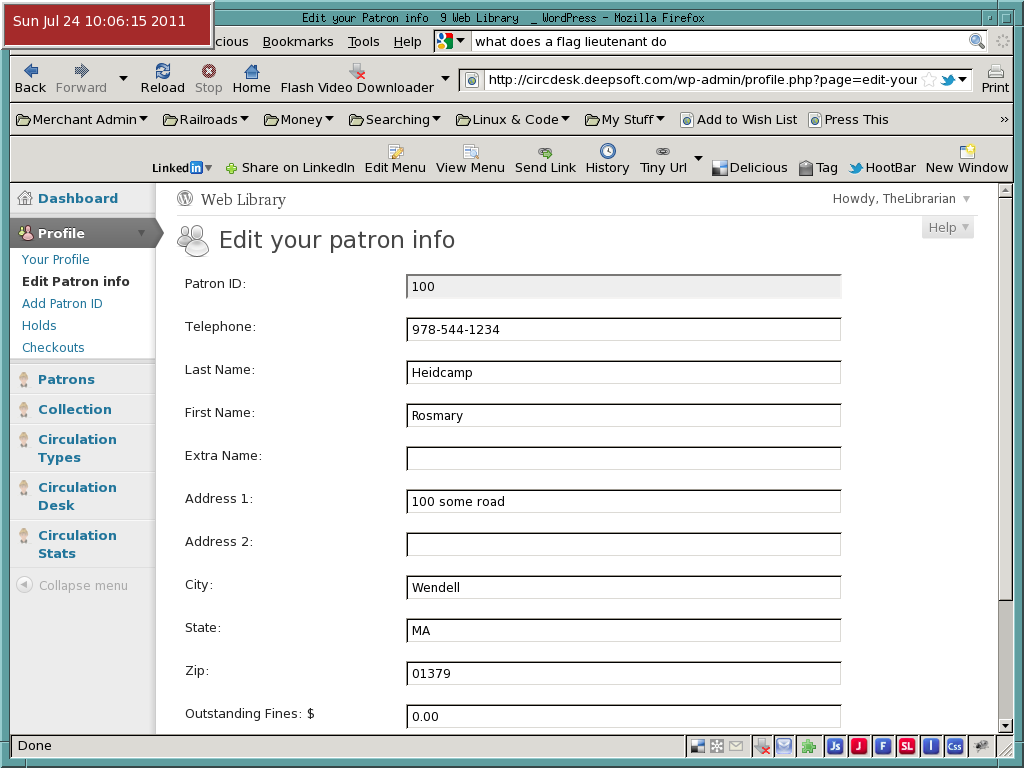
\includegraphics[width=4in]{EditPatronInfo.png}
\caption{Editing Patron Info}
\label{fig:EditPatronInfo}
\end{centering}
\end{figure}
This page, shown in Figure~\ref{fig:EditPatronInfo} allows WordPress
users to first associate their WordPress username with a patron id and
then allows them to update their name and contact information.

This form is also available for the front side via the short code
\textbf{weblib\_editpatroninfo}.

\subsection{Items on Hold}
This page lists the items a patron has requested a hold on.  The patron
can remove holds on selected items.

This page is also available on the front side with the short code 
\textbf{weblib\_editpatronholds}.

\subsection{Checked out items}
This page lists the items a patron has checked out. The due dates are
listed and the patron has the option of renewing items (up to a limit of
2 renewals).

This page is also available on the front side with the short code 
\textbf{weblib\_editpatroncircs}.

\subsection{Add Patron ID} This page, which requires priviledge
(\textbf{edit\_users}), allows librarians and administators to associate
(or disassociate) patron ids with WordPress users.

\section{Patron Management}

\begin{figure}[htbp]
\begin{centering}
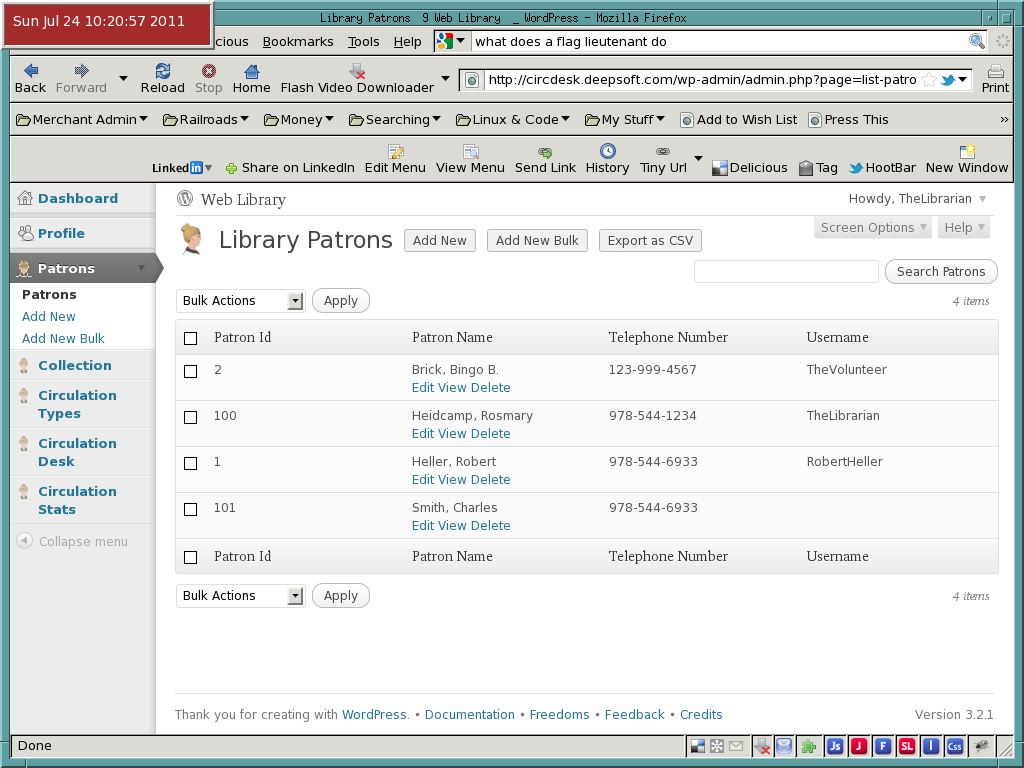
\includegraphics[width=4in]{PatronManagement.png}
\caption{Patron List Page}
\label{fig:PatronList}
\end{centering}
\end{figure}
Patron management entails the adding, removing, and editing of patrons
and requires \textbf{manage\_patrons} priviledge.  The main patron
management page, shown in Figure~\ref{fig:PatronList}, lists the
patrons in the database. Patrons can be added one at a time or in bulk.
Patrons can also be viewed or edited.  Each patron has a unique id
number, which is used when patrons either request holds or checkout
items.  Basic contact information is stored for each patron, as well as
any outstanding files.  Each patron also has an expiration date.
Nothing special is done when the expiration date is passed.  This is a
bookkeeping feature to allow librarians to cull inactive patrons.

The Patron database can be downloaded as a CSV file and Patrons can be
uploaded in bulk using a CSV file.  The columns recognized are:
\begin{description}
\item[id] The patron id.
\item[firstname] The patron's first name.
\item[lastname] The patron's last name.
\item[extraname] The patron's extra name (usually middle name).
\item[address1] The patron's first address line.
\item[address2] The patron's second (optional) address line.
\item[city] The patron's city.
\item[state] The patron's state.
\item[zip] The patron's zip code.
\item[telephone] The patron's telephone number.
\item[outstandingfines] The patron's outstanding fines.
\item[expiration] The patron's expiration date.
\end{description}

The minimum set of columns needed are \textbf{firstname},
\textbf{lastname}, \textbf{address1}, \textbf{city}, \textbf{state},
\textbf{zip}, and \textbf{telephone}.

\section{Collection Database Management}

\begin{figure}[htbp]
\begin{centering}
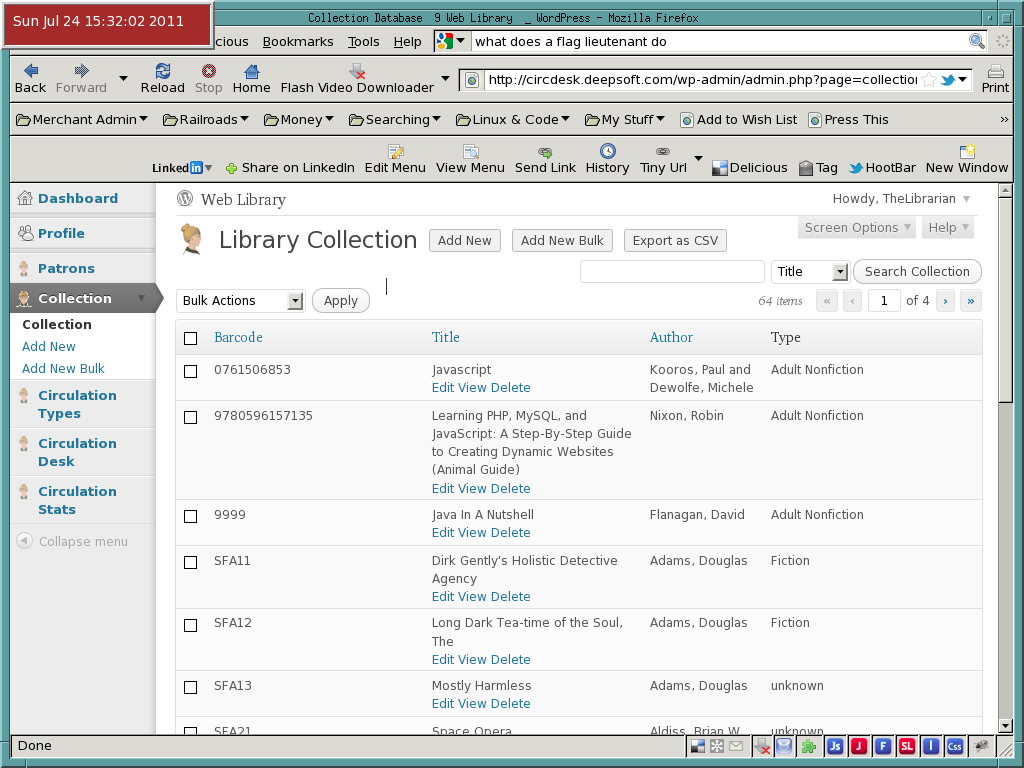
\includegraphics[width=4in]{ColectionListing.png}
\caption{Collection Listing Page}
\label{fig:CollectionList}
\end{centering}
\end{figure}
Collection database management entails the adding, removing, and
editing of items in your collection and requires
\textbf{manage\_collection} priviledge.  The main collection management
page, shown in Figure~\ref{fig:CollectionList}, lists the items in your
collection database. Items can be added one at a time or in bulk and
can be viewed or edited.  Each item has a unique ``barcode'', which is
up to 16 characters long.  Often this is a digit string as returned by
a barcode scanner, either from barcode stickers printed or purchased
for this purpose or from printed UPC labels on the items themselves.

Items in the collection database can be searched by title, author,
subject, ISBN, or keyword.  The rows can be worted by barcode, title, or
author. And the whole database can be exported as a CSV file.

\subsection{Adding and editing items in the collection database}

\begin{figure}[htbp]
\begin{centering}
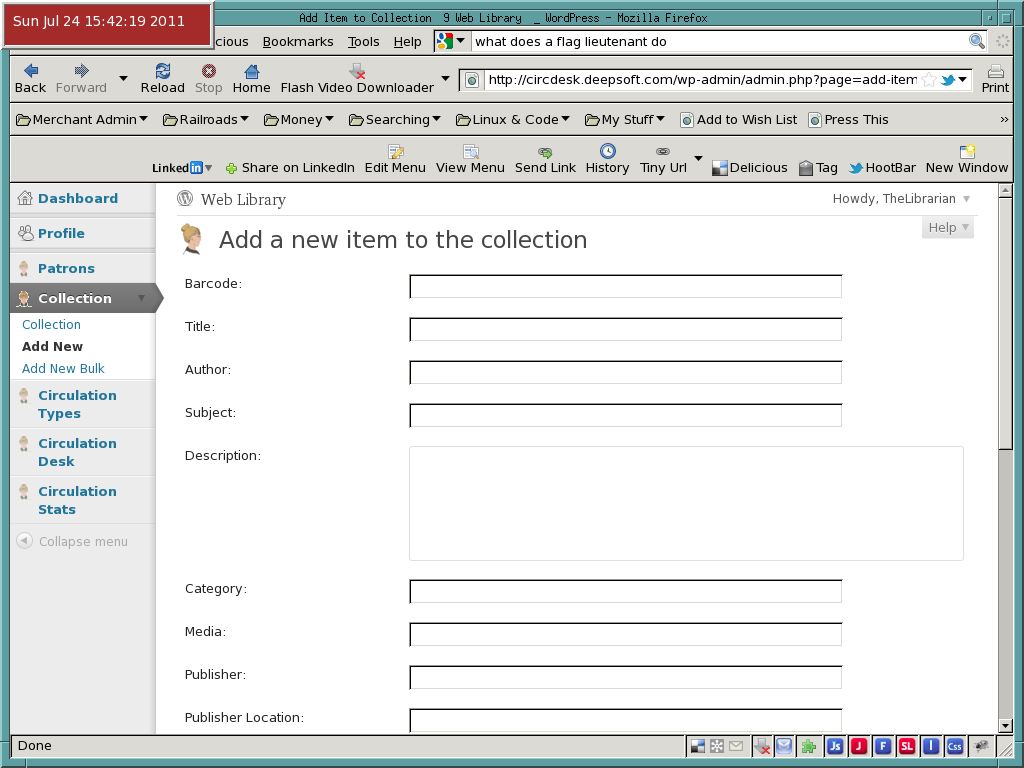
\includegraphics[width=4in]{AddItem.png}
\caption{Adding an item to the collection}
\label{fig:AddItem}
\end{centering}
\end{figure}
\begin{figure}[htbp]
\begin{centering}
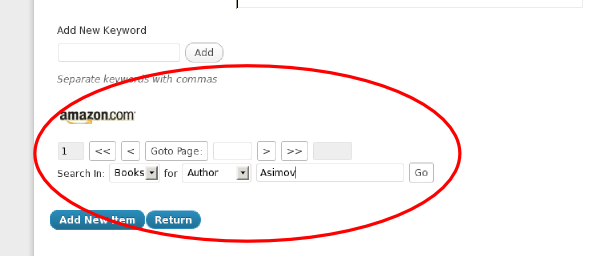
\includegraphics[width=4in]{AmazonSearch.png}
\caption{Amazon Search Form}
\label{fig:AmazonSearch}
\end{centering}
\end{figure}
\begin{figure}[htbp]
\begin{centering}
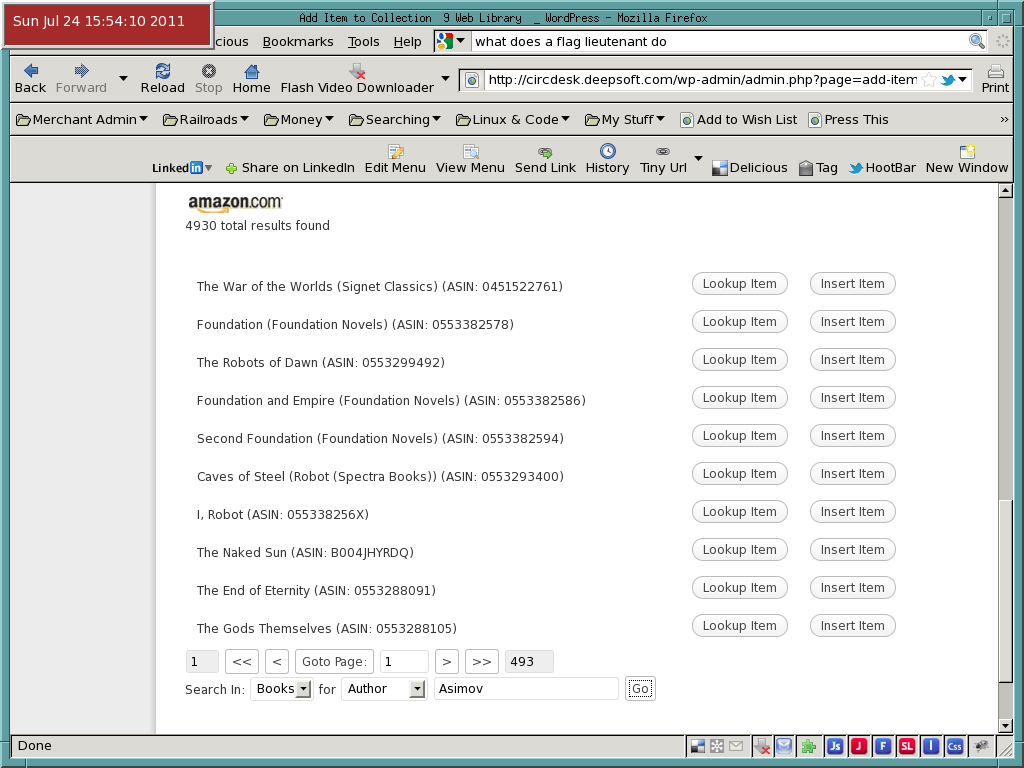
\includegraphics[width=4in]{AmazonSearchResults.png}  
\caption{Amazon Search Results}
\label{fig:AmazonSearchResults}
\end{centering}
\end{figure}
\begin{figure}[htbp]
\begin{centering}
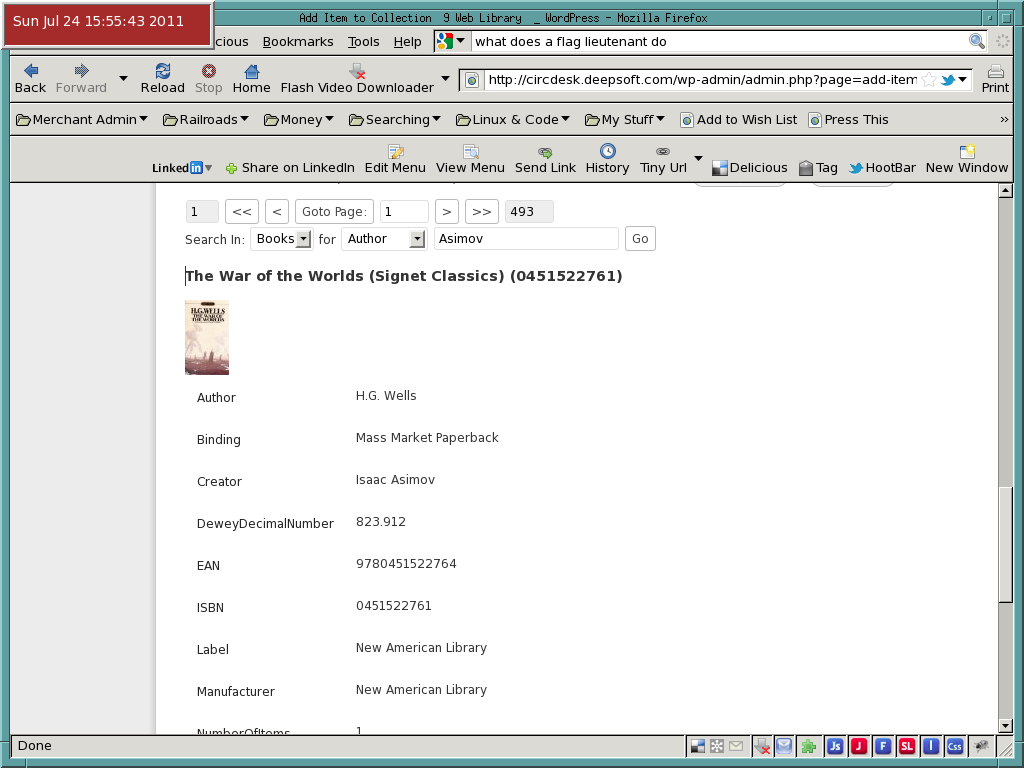
\includegraphics[width=4in]{AmazonLookupResults.png}  
\caption{Amazon Lookup Results}
\label{fig:AmazonLookupResults}
\end{centering}
\end{figure}
On the add item page, shown in Figure~\ref{fig:AddItem}, there are fields
for all of the database columns of an item, including Barcode, Title,
Author, Subject, Description, Category, Media, Publisher, Publisher
Location, Publish Date, Edition, ISBN, Type, Thumbnail URL, and
Keywords. Only the Title, Author, Subject, and Type are required.  It is
also possible to make use of Amazon's extensive product database to
find values for or to directly fill in these fields.  Under the Amazon
logo is a form for entering searches of Amazon's product database,
shown in Figure~\ref{fig:AmazonSearch}. Typical Amazon search results
are shown in Figure~\ref{fig:AmazonSearchResults} and item lookup
results are shown in Figure~\ref{fig:AmazonLookupResults}.

\clearpage

\subsection{Adding items in bulk to the collection database}

A CSV file can be uploaded to add items in bulk to the collection
database. The columns recognized are:

\begin{description}
\item[barcode] This is the item's barcode.
\item[title] This is the item's title. It is required.
\item[author] This is the item's author. It is required.
\item[subject] This is the item's subject. It is required.
\item[description] This is the item's description.
\item[category] This is the item's category.
\item[media] This is the item's media.
\item[publisher] This is the item's publisher.
\item[publocation] This is the item's publisher's location.
\item[pubdate] This is the item's publish date.
\item[edition] This is the item's edition.
\item[isbn] This is the item's ISBN.
\item[type] This is the item's type. It is required.
\item[thumburl] This is the item's thumbnail URL.
\item[keywords] This is the item's keywords (as a quoted, comma separated list).
\item[callnumber] This is the item's Call Number.
\end{description}  

\section{Circulation Type Management}

\begin{figure}[htbp]
\begin{centering}
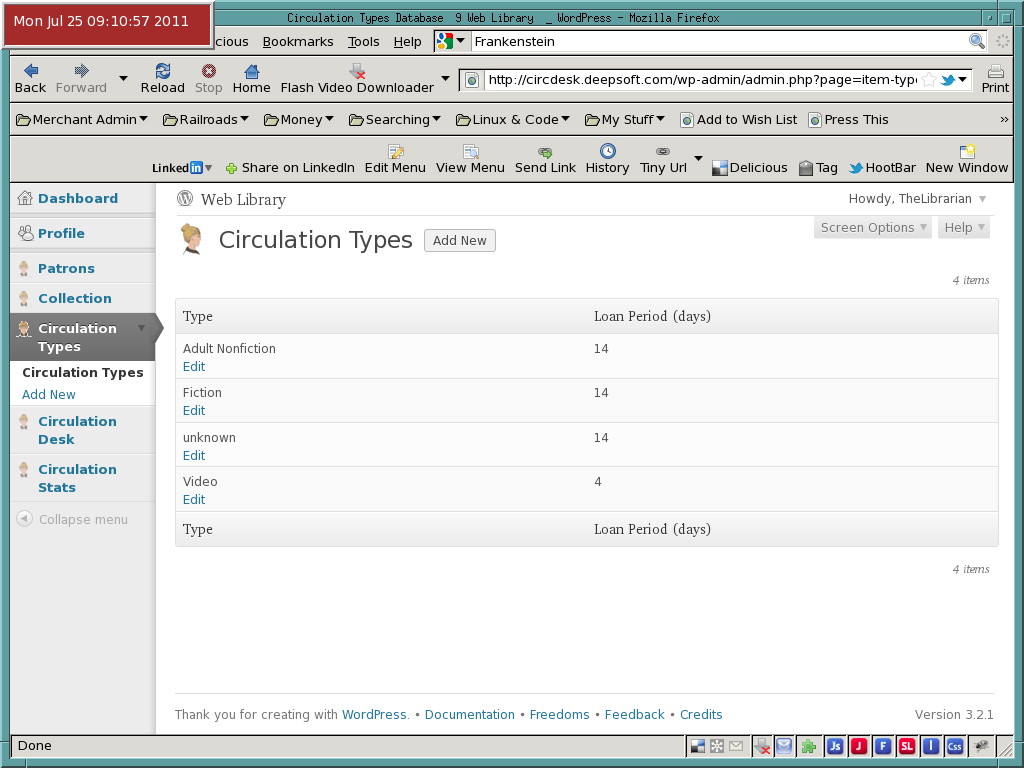
\includegraphics[width=4in]{CirculationTypesList.png}
\caption{Circulation Types List page}
\label{fig:CirculationTypesList}
\end{centering}
\end{figure}
Items in the collection database have an associated \textit{Circulation
Type}, which defines a loan period and is also used for statistical
anaylsis. The circulation type management pages are used to manage
these \textit{Circulation Types}, where they can be listed (see
Figure~\ref{fig:CirculationTypesList}, new ones added, and existing
ones edited.

\section{Circulation Desk}

The \textit{Circulation Desk} page implements a virtual circulation
desk, where circulation tasks can be performs.  These tasks consist of
checking out items, placing items on hold, checking in returns, listing
patron and item circulation records, listing items on hold, and listing
items checked out.  There are six aspects of this page, representing the
six functional modes:

\begin{enumerate}
\item \textbf{Main Circulation} This is the general entry mode, and
list all items in the collection with their circulation status,
described in Section~\ref{sect:MainCirculation}.
\item \textbf{Item Circulation Record} This mode list the circulation
status for a selected item in the collectection,
described in Section~\ref{sect:ItemCirculationRecord}.
\item \textbf{Patron Circulation Record} This mode lists the
circulation record for a selected patron.  This is a listing of items
this patron has on hold or has checked out, described in
Section~\ref{sect:PatronCirculationRecord}.
\item \textbf{Circulation Hold List} This mode lists the items that
currently have holds on them, described in
Section~\ref{sect:CirculationHoldList}.
\item \textbf{Circulation Checkout List} This mode lists the items that
are currently checked out, described in
Section~\ref{sect:CirculationCheckoutList}.
\item \textbf{Circulation Checkin Page} This mode is used for checking
in returned items, described in
Section~\ref{sect:CirculationCheckinPage}.
\end{enumerate}

\subsection{Main Circulation}
\label{sect:MainCirculation}

\begin{figure}[htbp]
\begin{centering}
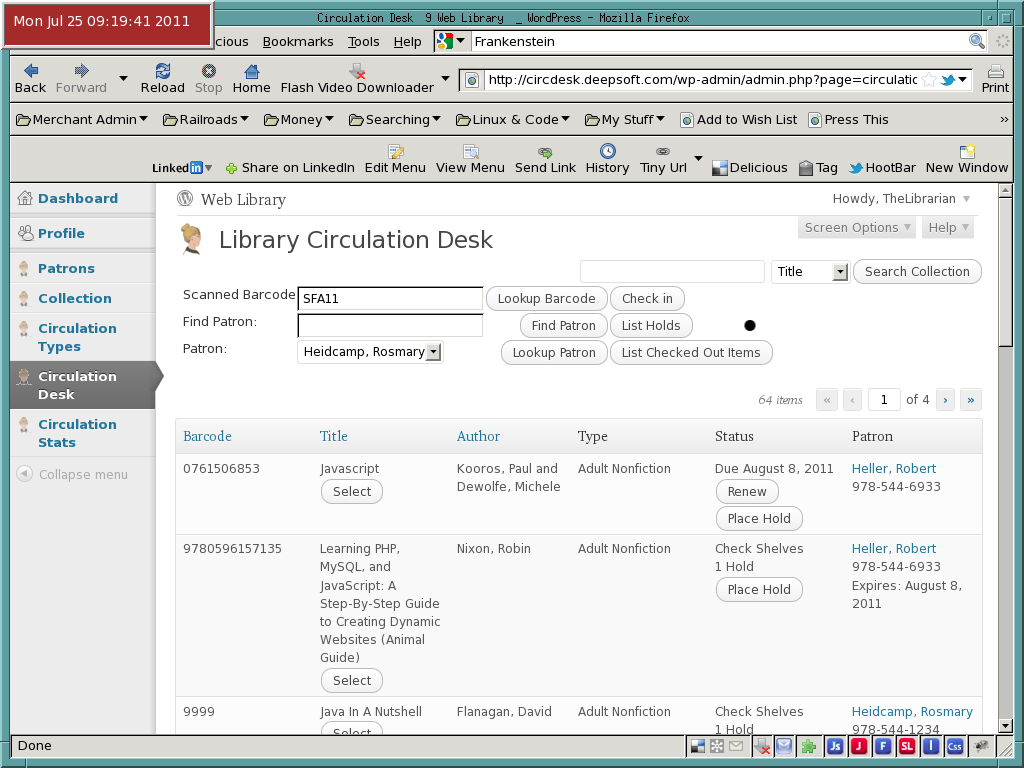
\includegraphics[width=4in]{MainCirculation.png}
\caption{Main Circulation page}
\label{fig:MainCirculation}
\end{centering}
\end{figure}
The main circulation page is the initial aspect of the \textit{Circulation
Desk} page. It lists the the circulation records of all
items\footnote{A page at a time.} in the collection.  The same searching
and ordering as is available on the collection management page is
available, as shown in Figure~\ref{fig:MainCirculation}.  From this aspect
all of the other aspects can be selected, by use of the various buttons
at the top of the page:
\begin{description}
\item[Lookup Barcode] This button looks up an item by barcode and
displays the selected items circulation record (see
Section~\ref{sect:ItemCirculationRecord}).
\item[Lookup Patron] This button looks up a selected patron and displays
the patron's circulation record (see
Section~\ref{sect:PatronCirculationRecord}). 
\item[Check in] This button shifts to the returned items check in page,
as described in Section~\ref{sect:CirculationCheckinPage}.
\item[List Holds] This button shifts to the circulation hold list
aspect, as described in Section~\ref{sect:CirculationHoldList}.
\item[List Checked Out Items] This button shifts to the circulation
checked out list, as described in Section~\ref{sect:CirculationCheckoutList}
\end{description}

\begin{figure}[htbp]
\begin{centering}
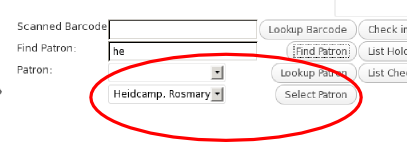
\includegraphics[width=4in]{FindPatron.png}
\caption{Patron Search Results}
\label{fig:FindPatron}
\end{centering}
\end{figure}
There is an additional button, the \textbf{Find Patron} button.  This
button does not change the page's aspect.  Instead it does a search, by
name, of the patron database and displays a drop down list of matches,
from which a patron can be selected, as shown in
Figure~\ref{fig:FindPatron}. 

All of the item lists are same\footnote{Except for the \textit{Patron
Circulation Record} listing, which ommits the \textbf{Patron} column.},
listing the item barcode, the item title, the item author, the item
status, and the patron the item is checked out to or held by. If the
item is neither checked out nor held, this last column is blank.  If an
item is both checked out and has a hold, the patron the item is checked
out to is listed.  If the item has more than one hold, the patron
associated with the first (earliest) hold is listed.  In the title
column is a \textbf{Select} button that can be used to directly look up
the item.  If the item is checked out, there will be a \textbf{Renew}
button in its status column.  There will always be a \textbf{Hold}
button in the status column, which will place a hold for the currently
selected patron.

\subsection{Item Circulation Record}
\label{sect:ItemCirculationRecord}

\begin{figure}[htbp]
\begin{centering}
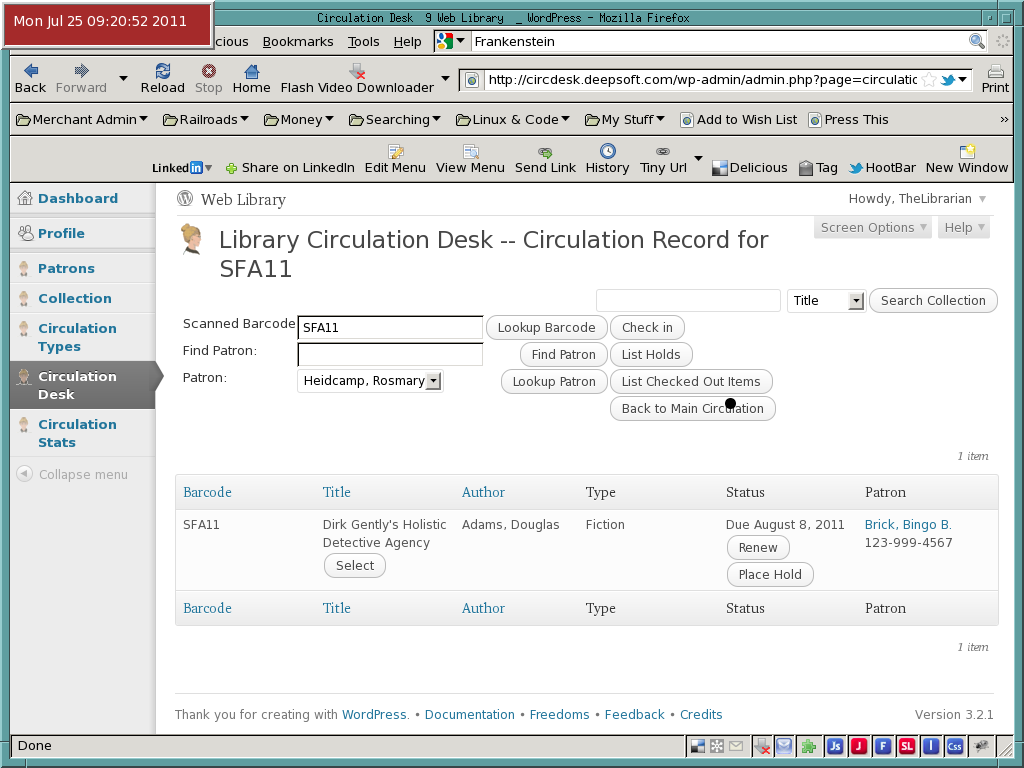
\includegraphics[width=4in]{ItemCirculationRecord.png}
\caption{Circulation Record for a selected item (SFA11)}
\label{fig:ItemCirculationRecord}
\end{centering}
\end{figure}
This aspect of the \textit{Circulation Desk} page is shown when a
specific item has been looked up or selected.  Only the selected item is
listed and an additional button is added to return to the main
aspect of the circulation desk page.  A typical view of this page is
shown in Figure~\ref{fig:ItemCirculationRecord}.

\subsection{Patron Circulation Record}
\label{sect:PatronCirculationRecord}

\begin{figure}[htbp]
\begin{centering}
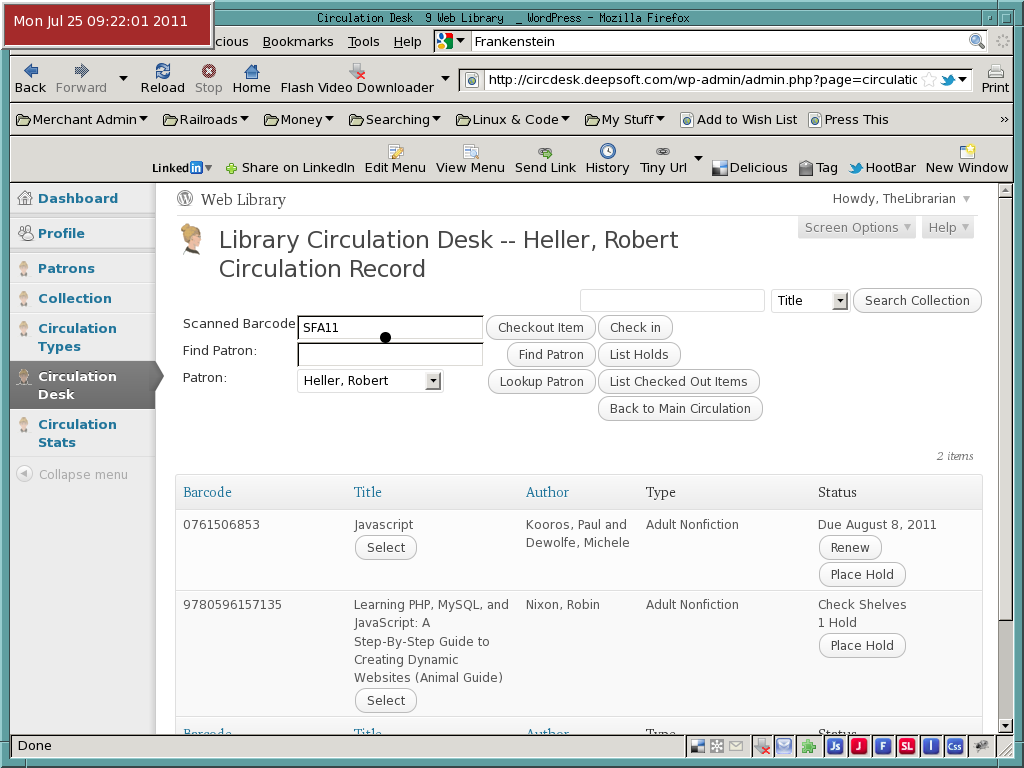
\includegraphics[width=4in]{PatronCirculationRecord.png}
\caption{Circulation Record for a selected patron (Heller, Robert)}
\label{fig:PatronCirculationRecord}
\end{centering}
\end{figure}
This aspect of the \textit{Circulation Desk} page is shown when a
selected patron is looked up.  It displays the selected patron's held
and checked out items.  The \textbf{Lookup Barcode} button is changed to
a \textbf{Checkout Item} button.  This button with cause the selected
item (barcode) to be checked out to the currently selected patron. 
Again, an additional button is added to return to the main
aspect of the circulation desk page.  A typical view of this page is
shown in Figure~\ref{fig:PatronCirculationRecord}.

\subsection{Circulation Hold List}
\label{sect:CirculationHoldList}

\begin{figure}[htbp]
\begin{centering}
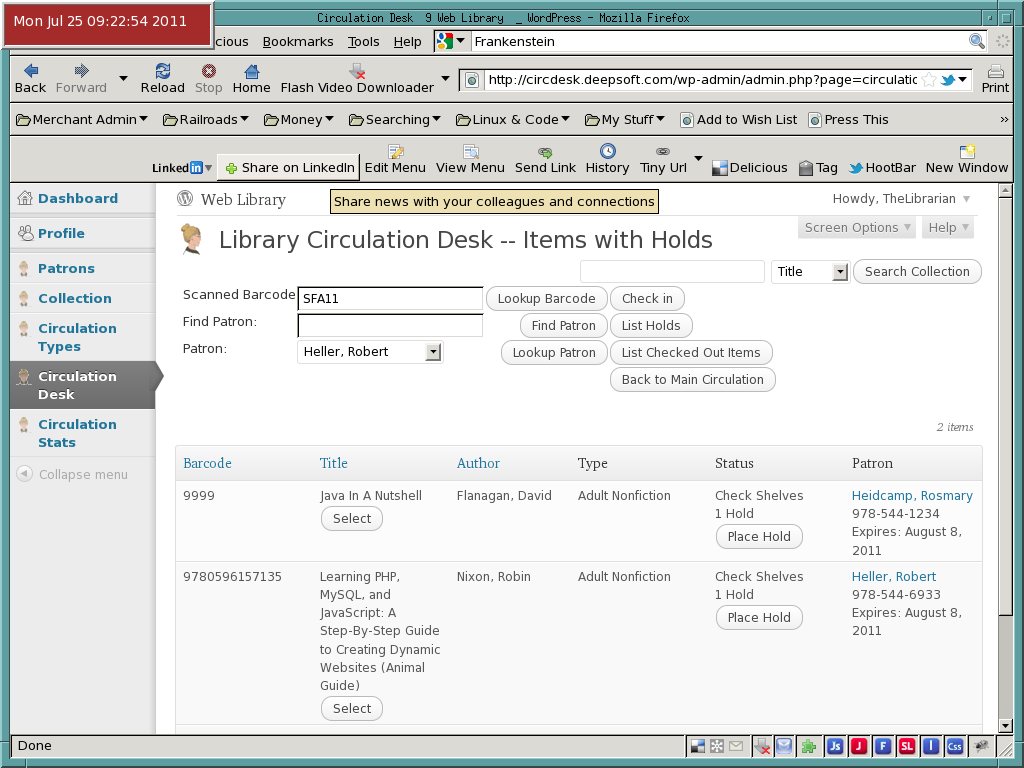
\includegraphics[width=4in]{CirculationHoldList.png}
\caption{Circulation Hold List}
\label{fig:CirculationHoldList}
\end{centering}
\end{figure}
This aspect of the \textit{Circulation Desk} page lists all items that
currently have holds on them. An additional button is added to return to
the main aspect of the circulation desk page.  A typical view of this
page is shown in Figure~\ref{fig:CirculationHoldList}.

\subsection{Circulation Checkout List}
\label{sect:CirculationCheckoutList}

\begin{figure}[htbp]
\begin{centering}
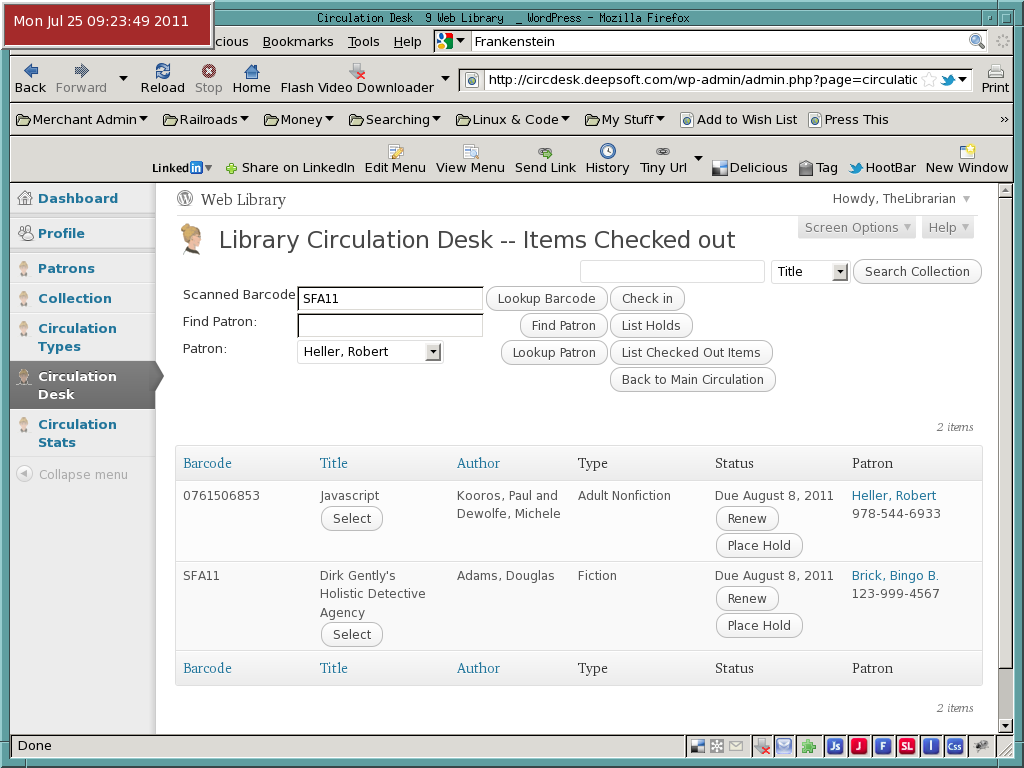
\includegraphics[width=4in]{CirculationCheckoutList.png}
\caption{Circulation Checkout List}
\label{fig:CirculationCheckoutList}
\end{centering}
\end{figure}
This aspect of the \textit{Circulation Desk} page lists all items that
are currently checked out. An additional button is added to return to
the main aspect of the circulation desk page.  A typical view of this
page is shown in Figure~\ref{fig:CirculationHoldList}.


\subsection{Circulation Checkin Page}
\label{sect:CirculationCheckinPage}

\begin{figure}[htbp]
\begin{centering}
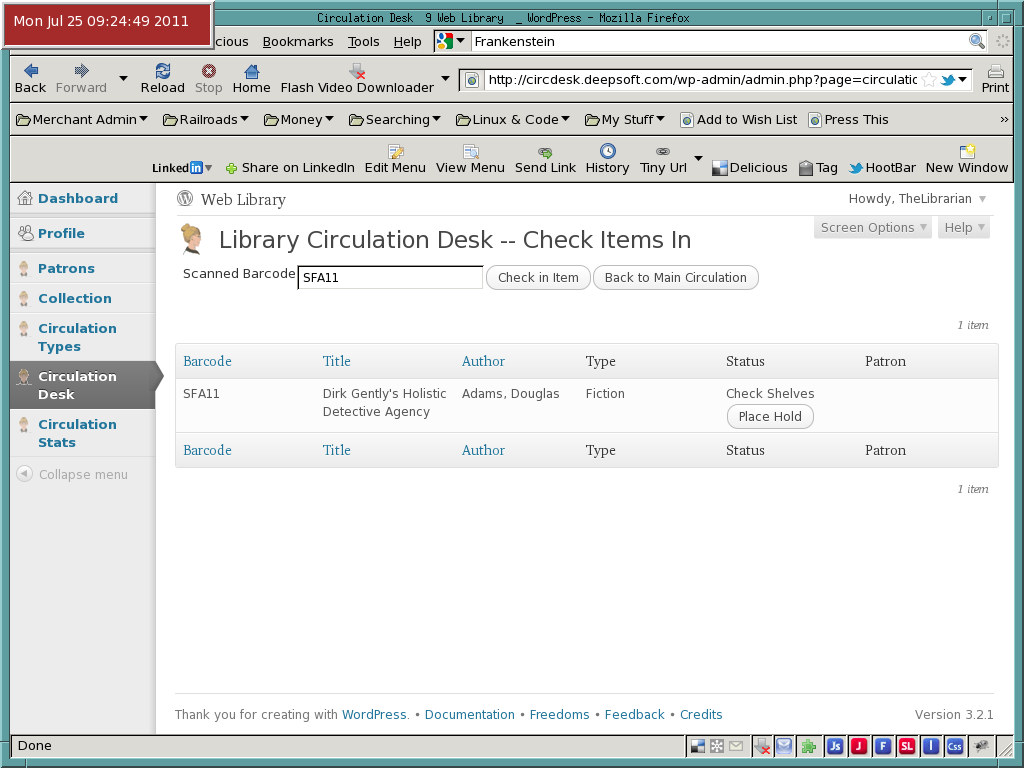
\includegraphics[width=4in]{CirculationCheckinPage.png}
\caption{Circulation Checkin Page}
\label{fig:CirculationCheckinPage}
\end{centering}
\end{figure}
This aspect of the \textit{Circulation Desk} is used to check in
returned items.  As items are checked in, they are listed as a
verification / sanity check. A button is provided to return to 
the main aspect of the circulation desk page.  A typical view of this   
page is shown in Figure~\ref{fig:CirculationCheckinPage}.

\section{Circulation Statistics}

\begin{figure}[htbp]
\begin{centering}
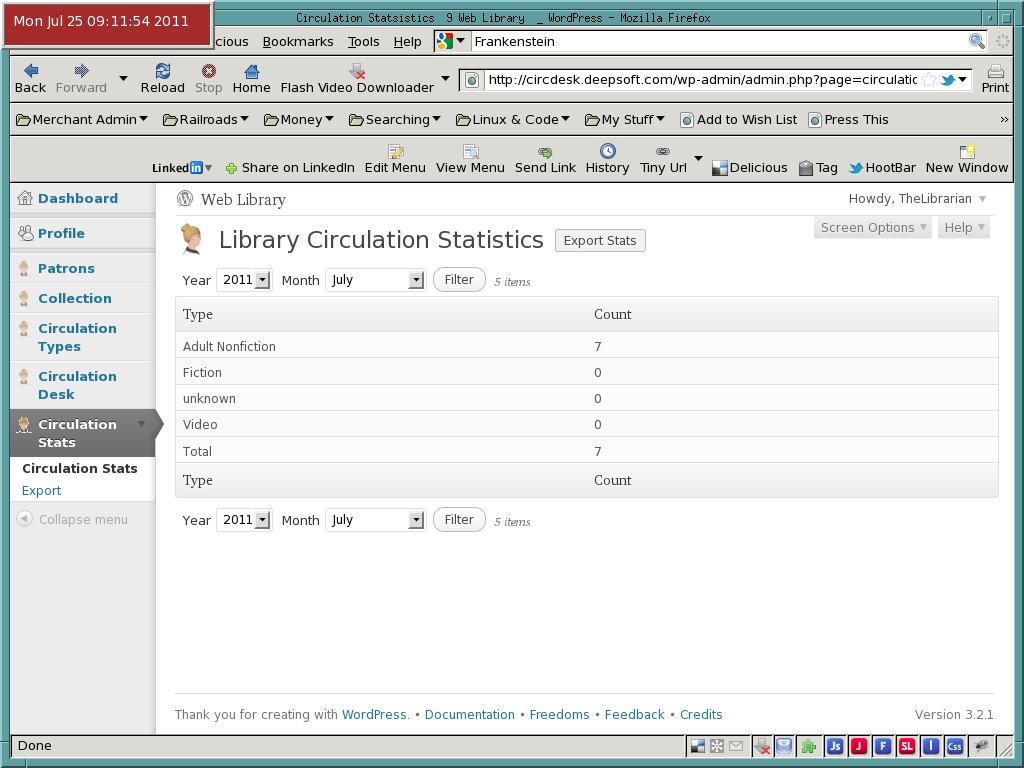
\includegraphics[width=4in]{CirculationTypesStatsList.png}
\caption{Circulation Types Statistics List page}
\label{fig:CirculationTypesStatsList}
\end{centering}
\end{figure}
Finally, circulation statistics can be viewed and downloaded using the
circulation statistics pages. Circulation statistics can be listed by
month (shown in Figure~\ref{fig:CirculationTypesStatsList}) or by
monthly totals.  The statistics can also be downloaded as CSV files.

\appendix

\section{Stylesheet selectors used by the short codes (front end).}

\begin{description}
\item[weblib-button] This selector is used with both input and a tags and 
defines how buttons look\footnote{With a (link) tags it makes the links look 
and act like buttons.}.

From \texttt{front.css}:

\begin{verbatim}
/* All <input type="submit" ...> and many <a href=""...> 
   have class="weblib-button" -- the links are meant to look 
   like buttons. I coded the submit buttons to have this 
   class as well as the <a href>'s, so that they would all 
   have the same styling. */

/* Common button styling */
.weblib-button {
  border: outset 2px #dcdad5;
  cursor: pointer;
  color: #000000;
  background-color: #dcdad5;
}

.weblib-button:hover {
  font-weight: normal;
  color: #000000;
  text-decoration: none;
}

/* Links-as-buttons styling */
a.weblib-button {
  height: 24px;
  white-space: nowrap;
  /*padding: 2px;*/
  padding: 0px;
/*  margin-top: 2px;
  margin-bottom: 2px;*/
}

a.weblib-button:link {
  font-weight: normal;
  color: #000000;
  text-decoration: none;
}

a.weblib-button:visited {
  color: #000000;
  font-weight: normal;
  text-decoration: none;
}
\end{verbatim}

\item[weblib-total-results] This selector is used with the total search 
results count.

From \texttt{front.css}:

\begin{verbatim}
.weblib-total-results {
  white-space: nowrap;
  font-weight: bold;
  font-size: 150%;
  float: left;
}
\end{verbatim}

\item[weblib-item-table] This selector is used with the tags that contain 
the search results.

From \texttt{front.css}:

\begin{verbatim}
.weblib-item-content-block, .weblib-item-table {
  display: table;
}
\end{verbatim}

\item[weblib-item-row] This selector is used with the tags that contain a 
row of search results.

From \texttt{front.css}:

\begin{verbatim}
.weblib-item-row {
  display: table-row;
  padding: 8px 0px;
  width: 100%;
}
\end{verbatim}

\item[weblib-item-index] This selector is used with the tag that contains the 
result index.

From \texttt{front.css}:

\begin{verbatim}
.weblib-item-index {
  font-size: 150%;
  padding: 0px 4px;
  text-align: left;
  width: 5%;
}
\end{verbatim}

\item[weblib-item-element] This is used with the tags for a single item 
element.

From \texttt{front.css}:

\begin{verbatim}
.weblib-item-element {
  display: table-cell;
  vertical-align: top;
  padding: 2px;
}
\end{verbatim}

\item[weblib-item-pagination-table] This is used with the pagination at the 
top and bottom of multipage results.

From \texttt{front.css}:

\begin{verbatim}
.weblib-item-pagination-table {
  display: table;
  width: 40%;
  margin: 2px 30%;
}
\end{verbatim}

\item[weblib-item-pagination] This is used with the pagination at the top and 
bottom of multipage results.

From \texttt{front.css}:

\begin{verbatim}
.weblib-item-pagination {
  display: table-row;
  width: 100%;
  padding: 8px 0px;
  font-size: 120%;
}

.weblib-item-pagination .pagelabel {
  vertical-align: top;
  display: table-caption;
  padding: 2px;
  font-weight: bold;  
}

.weblib-item-pagination .pagelink {
  vertical-align: top;
  display: table-cell;
  margin: 0px;
}

.weblib-item-pagination .pagenumform {
  white-space: nowrap;
  width: 25%;
}
\end{verbatim}

\item[weblib-item-long] This is used with long display of a single item.

From \texttt{front.css}:

\begin{verbatim}
.weblib-item-long {
  display: table;
}
\end{verbatim}

\item[weblib-item-head] This is the item heading styling.

\item[weblib-item-left] This is the left side of the long item display.

From \texttt{front.css}:

\begin{verbatim}
.weblib-item-left {
  width: 90%;
}
\end{verbatim}

\item[weblib-item-content-block] This is the long item content block.

From \texttt{front.css}:

\begin{verbatim}
.weblib-item-content-block, .weblib-item-table {
  display: table;
}
\end{verbatim}

\item[weblib-item-content-element] This is the long item content element.

From \texttt{front.css}:

\begin{verbatim}
.weblib-item-content-element {
  display: table-row;
}
\end{verbatim}

\item[weblib-item-left-head] This is the long item left heading.

From \texttt{front.css}:

\begin{verbatim}
.weblib-item-left-head {
  font-weight: bold;
  text-align: right;
  display: table-cell;
  padding: 2px;
}
\end{verbatim}

\item[weblib-item-left-content] This is the long item left content.

From \texttt{front.css}:

\begin{verbatim}
.weblib-item-left-content {
  text-align: left;
  display: table-cell;
  padding: 2px;
}
\end{verbatim}

\item[weblib-item-author] This is the styling of the author name.

From \texttt{front.css}:

\begin{verbatim}
.weblib-item-author {
  text-decoration: underline;
}
\end{verbatim}

\item[weblib-item-title] This is the styling of the title.

From \texttt{front.css}:

\begin{verbatim}
.weblib-item-title {
  font-weight: bold;
}
\end{verbatim}

\item[weblib-item-right] This is the styling of the right side of the long 
item display.

From \texttt{front.css}:

\begin{verbatim}
.weblib-item-right {
}
\end{verbatim}

\item[weblib-item-center-head] This is the styling of the keyword heading of
the heading.

From \texttt{front.css}:

\begin{verbatim}
.weblib-item-center-head {
  font-weight: bold;
  text-align: center;
  display: table-cell;
  padding: 2px;
}
\end{verbatim}

\item[weblib-item-keyword-list] This is the styling of the keyword list.

From \texttt{front.css}:

\begin{verbatim}
.weblib-item-keyword-list {
  text-align: center;
  display: table-cell;
  padding: 2px;
}
\end{verbatim}

\item[weblib-item-thumb] This is the styling of the thumbnail image.

From \texttt{front.css}:

\begin{verbatim}
.weblib-item-thumb {
  padding: 0px 4px;
}

.weblib-item-thumb img {
  min-width: 48px;
  min-height: 72px;
}
\end{verbatim}

\item[weblib-item-holdbutton] This is the styling of the hold (request) 
button.

From \texttt{front.css}:

\begin{verbatim}
.weblib-item-holdbutton {
}
\end{verbatim}

\item[weblib-item-brief] This is used to style the brief item display.

From \texttt{front.css}:

\begin{verbatim}
.weblib-item-brief {
}
\end{verbatim}

\item[weblib-item-info] This is used to style the item info.

From \texttt{front.css}:

\begin{verbatim}
.weblib-item-info {
  width: 85%;
}
\end{verbatim}
\end{description}

\end{document}

